\section{Durchführung}
\subsection{Aufbau}
Der Versuch besteht aus einem Ultraschall-Doppler-Generator, der sich im Pulsbetrieb befindet, einer Ultraschallsonde, die eine Frequenz
von \qty{2}{\mega\hertz} aussendet, und einem Rechner zur Datenaufnahme und -analyse.
Es wird eine Strömungsröhre mit einem Innendurchmesser von \qty{10}{\milli\meter} und einem Außendurchmesser von \qty{15}{\milli\meter}
untersucht.
Die verwendete Flüssigkeit ist ein Gemisch aus Wasser, Glycerin und Glaskugeln.
Dabei ist die Viskosität des Gemisches so gewählt, dass bei mittlerer Strömungsgeschwindigkeit eine laminare Strömung vorhanden ist.
Die Flüssigkeit hat dabei eine Dichte von \qty{1.15}{\gram\per\cubic\centi\meter} und eine Viskosität von \qty{12}{\milli\pascal\second}. 
Die Strömungsgeschwindigkeit selbst kann dabei zwischen 0 und \qty{7.5}{\liter\per\minute} eingestellt werden.
Ferner gibt es ein Doppler-Prisma aus Acryl, das die drei Einschallwinkel $\theta =$ \qty{15}{\degree}, \qty{30}{\degree} und \qty{60}{\degree} hat,
vgl. Abbildung \ref{fig:prisma}.
Der Dopplerwinkel $\alpha$ kann gemäß
\begin{align}
    \alpha = \qty{90}{\degree} - \arcsin\left(\sin\theta \cdot \frac{c_\text{L}}{c_\text{P}}\right)
    \label{eq:dopplerwinkel}
\end{align}
berechnet werden, wobei $c_\text{L} = \qty{1800}{\meter\per\second}$ und $c_\text{P} = \qty{2700}{\meter\per\second}$ jeweils die 
Schallgeschwindigkeit in der Flüssigkeit bzw. dem Prisma sind.
Alle drei Auflageflächen haben den gleichen Abstand von \qty{30.7}{\milli\meter} zwischen Sonde und Flüssigkeit.
Die verschiedenen Winkel dienen dem Zwecke der Reproduzierbarkeit.
Um Verluste beim Übergang zwischen Sonde und Prisma bzw. Prisma und Rohr zu vermeiden, steht ein Kontaktgel zu Verfügung.
In Abbildung \ref{fig:prisma} ist außerdem erkennbar, dass das Prisma eine Aussparung für eine Platte hat, mit der das Rohr auf der richtigen
Höhe für das Prisma gehalten werden kann.

\begin{figure}[H]
    \centering
    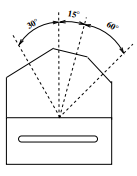
\includegraphics[height = 5 cm]{Abbildungen/prisma.png}
    \caption{Ein Doppler-Prisma \cite{man:us3}.}
    \label{fig:prisma}
\end{figure}


\subsection{Messprogramm}
\subsubsection{Messreihe zur Bestimmung der Geschwindigkeit der Glaskugeln}
Zur Messung der Strömungsgeschwindigkeit der Kugeln in Abhängigkeit des Dopplerwinkels und der Flussgeschwindigkeit wird am 
Ultraschallgenerator der Regler \texttt{SAMPLE VOLUME} auf \texttt{LARGE} gestellt.
Für insgesamt 5 Flussgeschwindigkeiten wird die Frequenzverschiebung bei jedem Dopplerwinkel gemessen.


\subsubsection{Messreihe zur Untersuchung des Strömungsprofils}
Für den Prismawinkel von \qty{15}{\degree} wird bei einer einer Pumpleistung von \qty{5}{\liter\per\minute} und \qty{3}{\liter\per\minute}
die Strömungsgeschwindigkeit und der Streuintensitätswert (als Maß für den Dopplerwinkel) gemessen.
Dies entspricht ca. $67 \, \%$ bzw. $40 \, \%$ der maximalen Leistung.
Die beiden Größen werden in Abhängigkeit der Tiefe gemessen.





\section{Vorbereitungsaufgabe}
Gemäß Gleichung \eqref{eq:dopplerwinkel} kann der Dopplerwinkel in Abhängigkeit von $\theta$ bestimmt werden.
Mit Hilfe der oben angegebenen Werte ergibt sich dann Tabelle \ref{tab:vorbereitung}.

\begin{table}[H]
    \centering
    \caption{Der Dopplerwinkel $\alpha$ in Abhängigkeit des Prismawinkels $\theta$.}
    \label{tab:vorbereitung}
    \sisetup{table-format=2.0}
    \begin{tabular}{
        S % prismawinkel
        S % dopplerwinkel
    }
    \toprule
    {$\theta / \unit{\degree}$} & {$\alpha / \unit{\degree}$} \\
    \midrule 
    15 & 80 \\
    30 & 71 \\
    60 & 55 \\
    \bottomrule
    \end{tabular}
\end{table}
% huhu you are doing great :D